\section{Options and Tail Risk}

A particularly interesting example of tail risk comes from put options on market indices, whose payoffs make tail risk and potential mispricing visible at a glance. 

\subsection{Options Background}
A put option gives the holder the right to sell a security for a fixed amount, $K$ (the exercise/strike price). \autoref{fig:fig10}(a) shows the payoff for buying (or going long) a put option at maturity as a function of the price of the underlying security at expiry, $S_1$. Conversely, \autoref{fig:fig10}(b) shows the other side of the options contract (i.e., writing or shorting a put option). 

\begin{figure}[h]
    \centering
    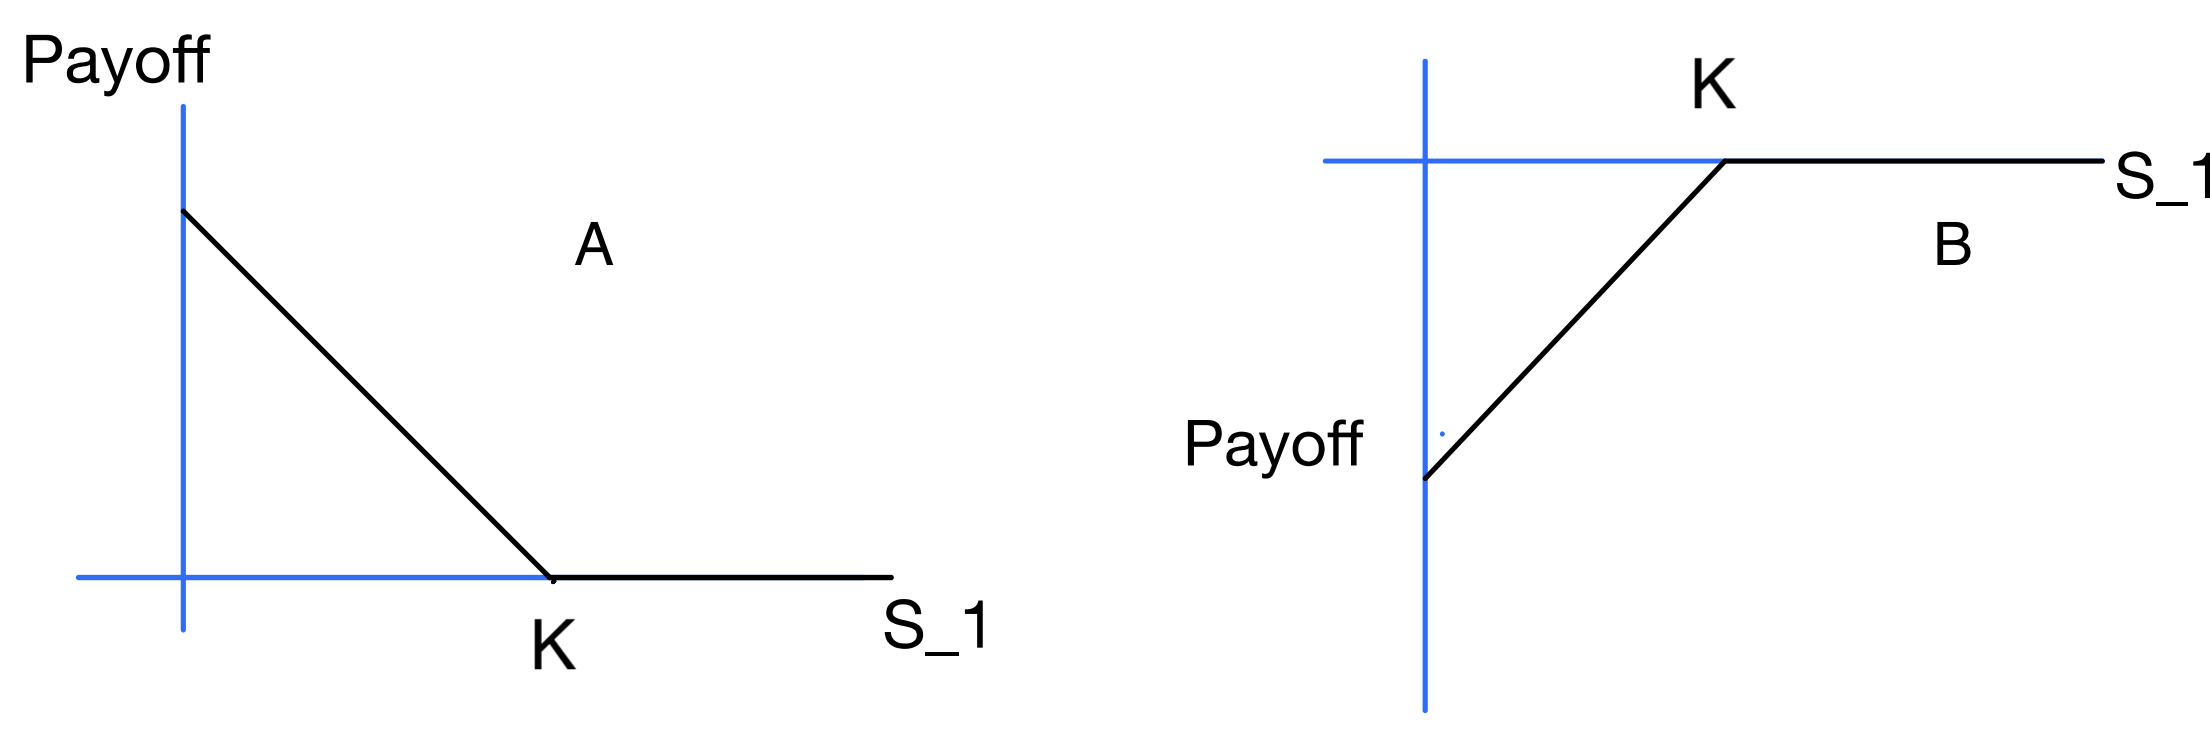
\includegraphics[width=0.50\textwidth]{fig10.png}
    \caption{Payoffs for long and short put options}
    \label{fig:fig10}
\end{figure}

The payoff for buying a put option is $max(K - S_1, 0)$. When $S_1 \ge K$, the option is considered out-of-the-money (OTM). The payoff of an OTM put is $0$ because one would not exercise the option. When $S_1 < K$, the option is considered in-the-money. The payoff for the buyer is $K-S_1$, and the writer of the option is forced to buy the security for more than it is worth. Thus, the put option’s seller insures the buyer against the underlying’s price decline. 

This payoff structure introduces negative skewness for the writer. Most of the time ($S_1 \ge K$), the writer will pay out zero, whereas only some of the time ($S_1 < K$) the writer will pay out something positive. Because of this negative skew, the writer of the option earns a \say{premium} ($p$), the positive amount that the options buyer pays. Thus, when writing puts on broad market indices, the strategy initially appears attractive since large market crashes are relatively rare events. The actual payoff for a put option writer is $- max(K-S_1, 0) + p$. While this sounds promising because the writer earns $p$ most of the time, the market can sometimes crash (i.e., $S_1 << K$), leading to significant losses for the writer.

The Black-Scholes model (BSM), initially published in 1973, provides a framework to determine the fair value of this premium $p$ \citep{black1973pricing}. The core of the model is a simple binomial tree (\autoref{fig:fig11}). As one holds the the maturity of an option constant and increases the number of steps within the binomial tree, by the central limit theorem, the distribution of returns approaches a lognormal one \citep{cox1979option}.

\begin{figure}[h]
    \centering
    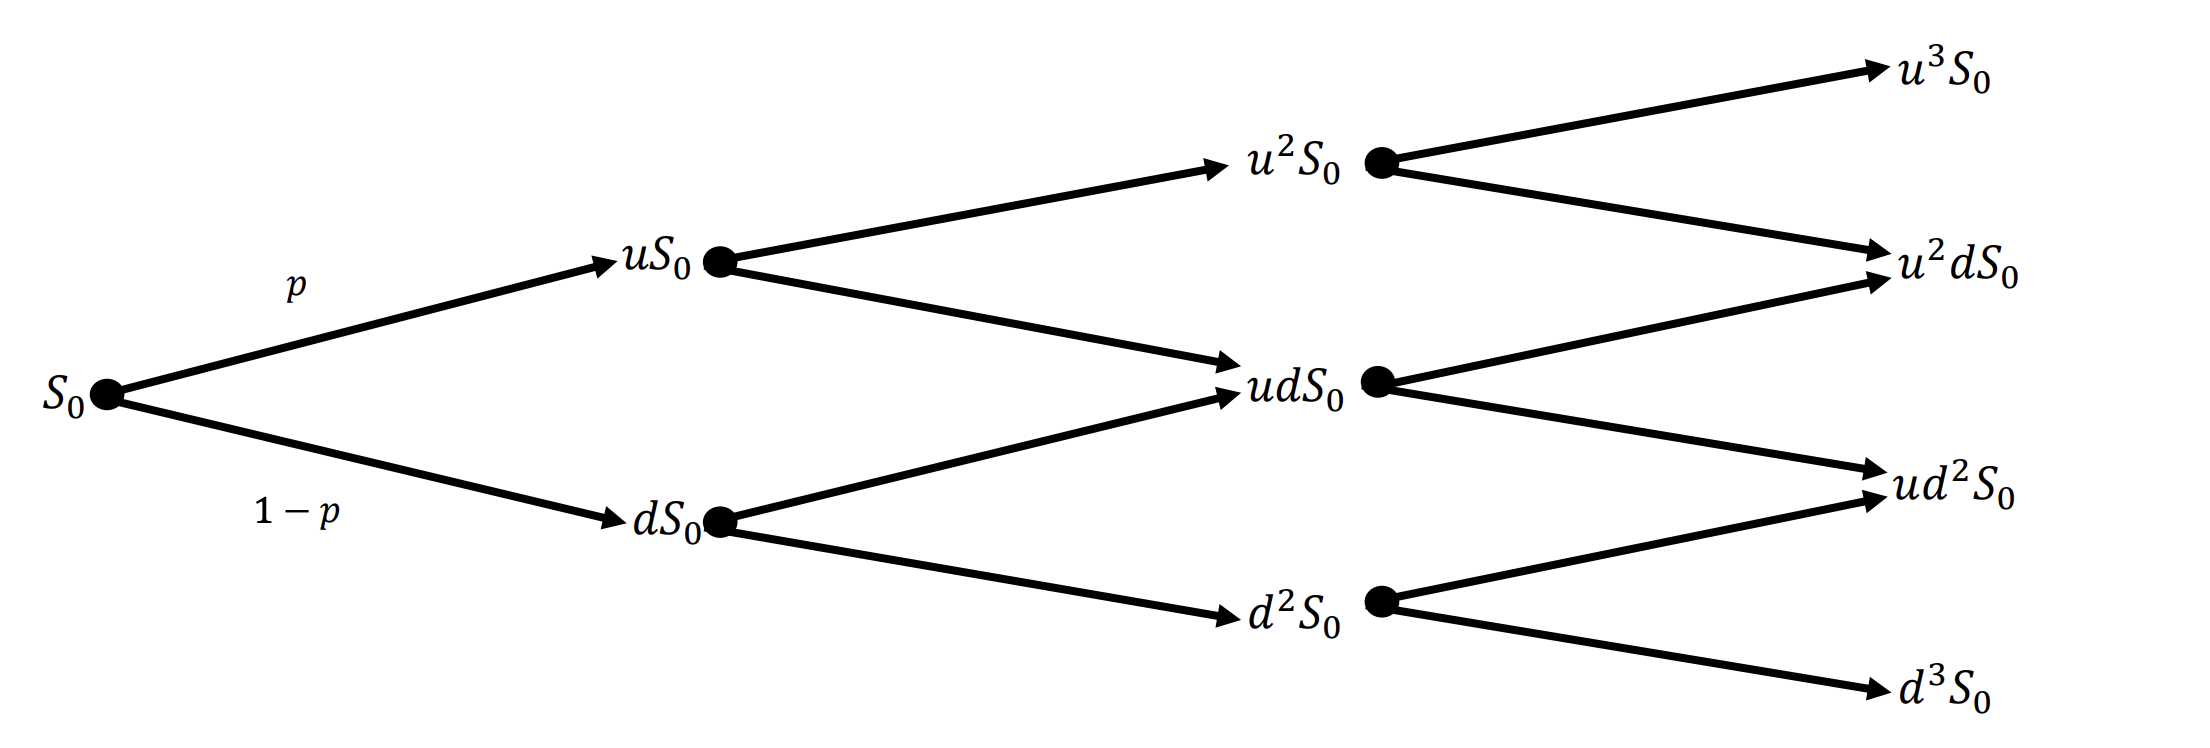
\includegraphics[width=0.75\textwidth]{fig11.png}
    \caption{Binomial tree}
    \label{fig:fig11}
\end{figure}

Black, Scholes, and Merton showed that the price of the option depends on the current value of the underlying ($S_0$; also known as spot price), exercise price ($K$), time to maturity, interest rate (risk-free rate), and volatility \citep{black1973pricing, merton1971theory}. All are directly observable except the volatility. Given an actual option price, it is possible to back out the volatility (called “implied volatility”). Since actual option prices reflect market participants’ expectation and risk preferences, this implied volatility is the market’s risk-neutral expectation of future price volatility.

If the market priced options as if the lognormal distribution were true, then implied volatility would match realized volatility, and as such, would not differ between options of different strike prices. In the initial years following the model’s publication, empirical evidence largely supported this theoretical prediction. However, the market crash of October 19, 1987, marked a structural deviation. 


\subsection{The 1987 Crash}
\autoref{fig:fig12}(a) \citep{benzoni2011explaining} shows the time series of the difference between implied volatility for at-the-money (ATM) and OTM 1-month put options. Specifically, this measures ${IV}_{10\% OTM} - {IV}_{ATM}$, where the OTM put has a strike price $10\%$ below the current underlying price ($K = 0.90 \cdot S_0$).

\begin{figure}[h]
    \centering
    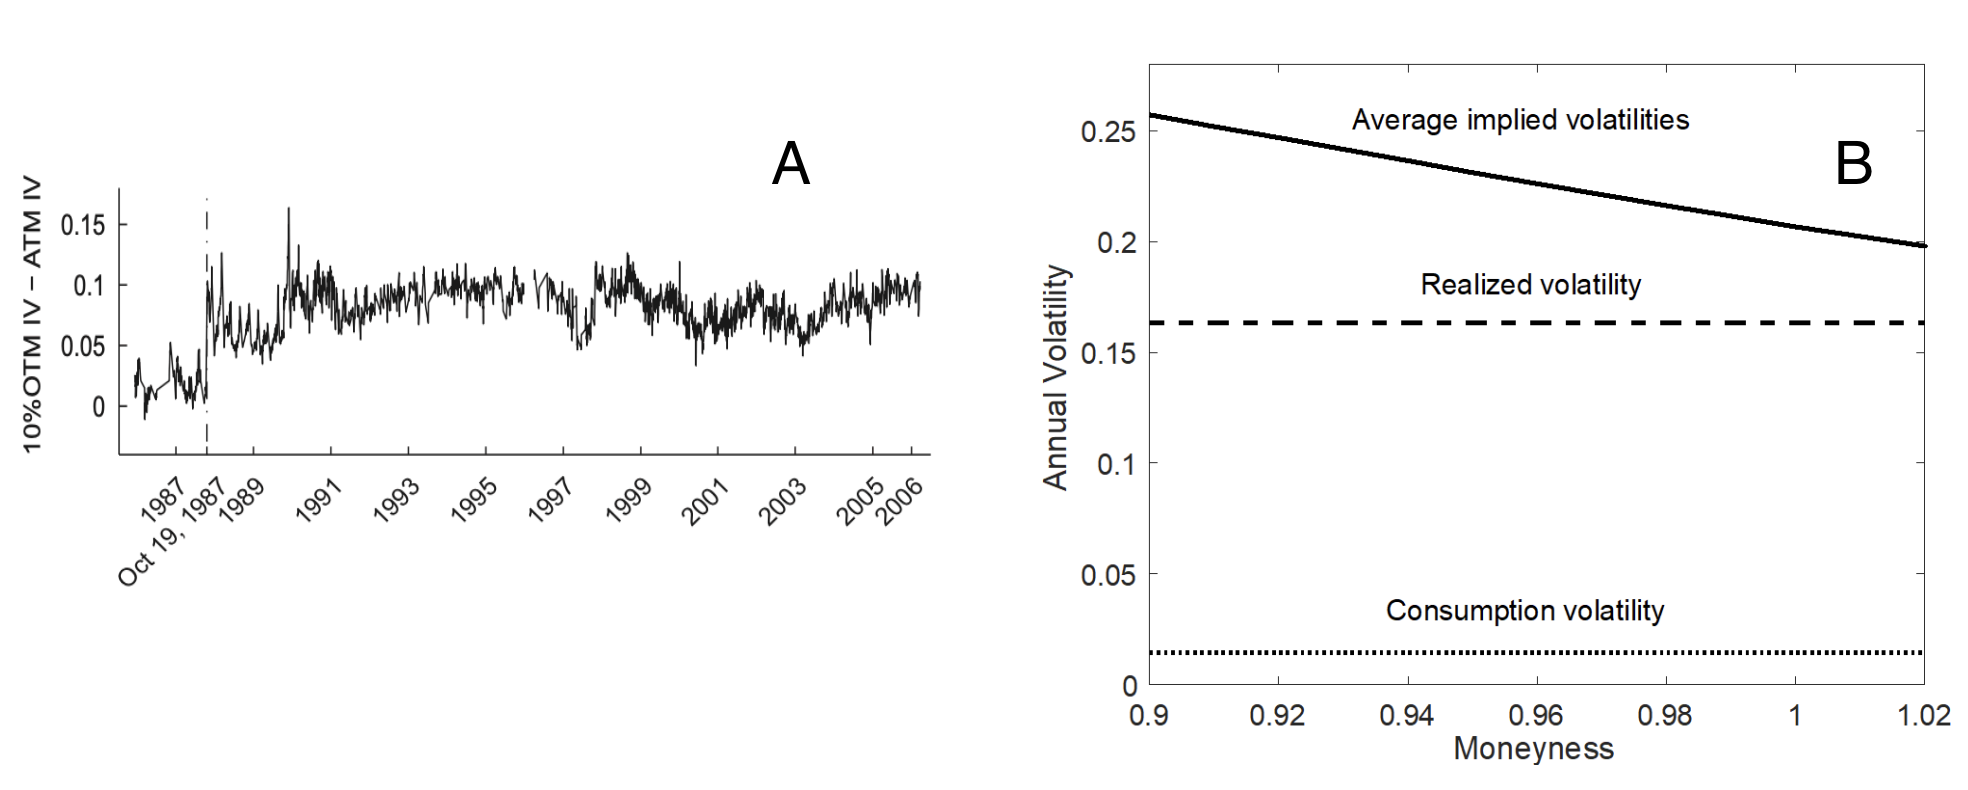
\includegraphics[width=0.75\textwidth]{fig12.png}
    \caption{Volatility skew before and after 1987 \citep{benzoni2011explaining, seo2019option}}
    \label{fig:fig12}
\end{figure}

Before October 19, 1987, the spread fluctuated around zero, indicating a flat implied volatility surface across all strikes consistent with BSM’s lognormal assumption. However, following the crash, the spread widened out and has remained wide to this day, showing that investors have since paid an ever-larger volatility premium for downside insurance.

What made October 19, 1987 so significant? The daily returns implied a 20 standard deviation event under the normal distribution assumption. To put this in perspective, the chance of an event beyond ten standard deviations is less than ${10}^{-30}$\textemdash an unimaginably small number. In the world of continuous diffusion processes underlying BSM, such an event has zero probability. For finance specialists, this meant that the supposedly arbitrage-free Black-Scholes model actually contained arbitrage opportunities after all.

This crash revealed a fundamental problem: model risk. In 1987, options traders discovered that they were using an incorrect model. This exposes two types of uncertainty. One is internal to the model, such as extreme but still-possible paths in a binomial tree. The other lies outside the model’s domain—events that the model cannot imagine. The 1987 crash was clearly the latter.

\autoref{fig:fig12}(b) \citep{seo2019option} shows how the market adapted post-crash. The figure displays average implied volatility for one-month index options as a function of \say{moneyness} (defined as the strike-to-spot ratio, $\frac{K}{S_0}$). When $\frac{K}{S_0} < 1$, the put is OTM. The downward-sloping curve shows that deeper OTM puts carry increasingly higher implied volatilities. 

This pattern reflects investors' willingness to pay higher "insurance premiums" for protection against large losses. Post-1987, the market assigns greater probability to extreme downward moves than a lognormal distribution would predict. The volatility skew has become a direct measure of tail risk concern, showing that investors now systematically overprice downside protection relative to BSM's theoretical predictions.

Why did market participants fail to incorporate tail risk into option pricing despite historical precedent? The 1929 crash (almost exactly 58 years prior to the 1987 crash) provided clear evidence against normality, yet it was largely ignored. Perhaps the $1980s$ marked the beginning of widespread quantitative modeling in finance (coming soon after BSM's publication) when practitioners had limited historical data and may have suffered from small sample bias in estimating tail probabilities.

\subsection{The Chicken Problem}
Some types of uncertainty and distributions (like the short put strategy and those with fat tails) seem destined to fool us. 

Bertrand Russell observed, \say{The man who has fed the chicken every day throughout its life at last wrings its neck instead, showing that more refined views as to the uniformity of nature would have been useful to the chicken} \citep{russell1912induction}. Bertrand Russell’s chicken is often used to invoke the failure of empiricism and inductivism. The chicken is not helped at all by having a long time series of observations. 

Writing put options exemplifies this chicken problem well. \autoref{fig:fig13} compares daily returns from the market portfolio (discussed in Section $4.1$) and a put-write strategy using CBOE data. Data on the put-writing strategy was collected from CBOE's S\&P 500 PutWrite Index, which tracks a hypothetical portfolio combining Treasury bills with short positions in at-the-money S\&P 500 put options \citep{Cboe}.

\autoref{fig:fig13} displays the stock‑market data in red, the unlevered short‑put strategy in blue, and their overlap in purple. The put-write strategy return has a similar mean but a much smaller variance and is highly concentrated at its mean. The many positive, low volatility returns can lure investors into believing in safety. 

\begin{figure}[h]
    \centering
    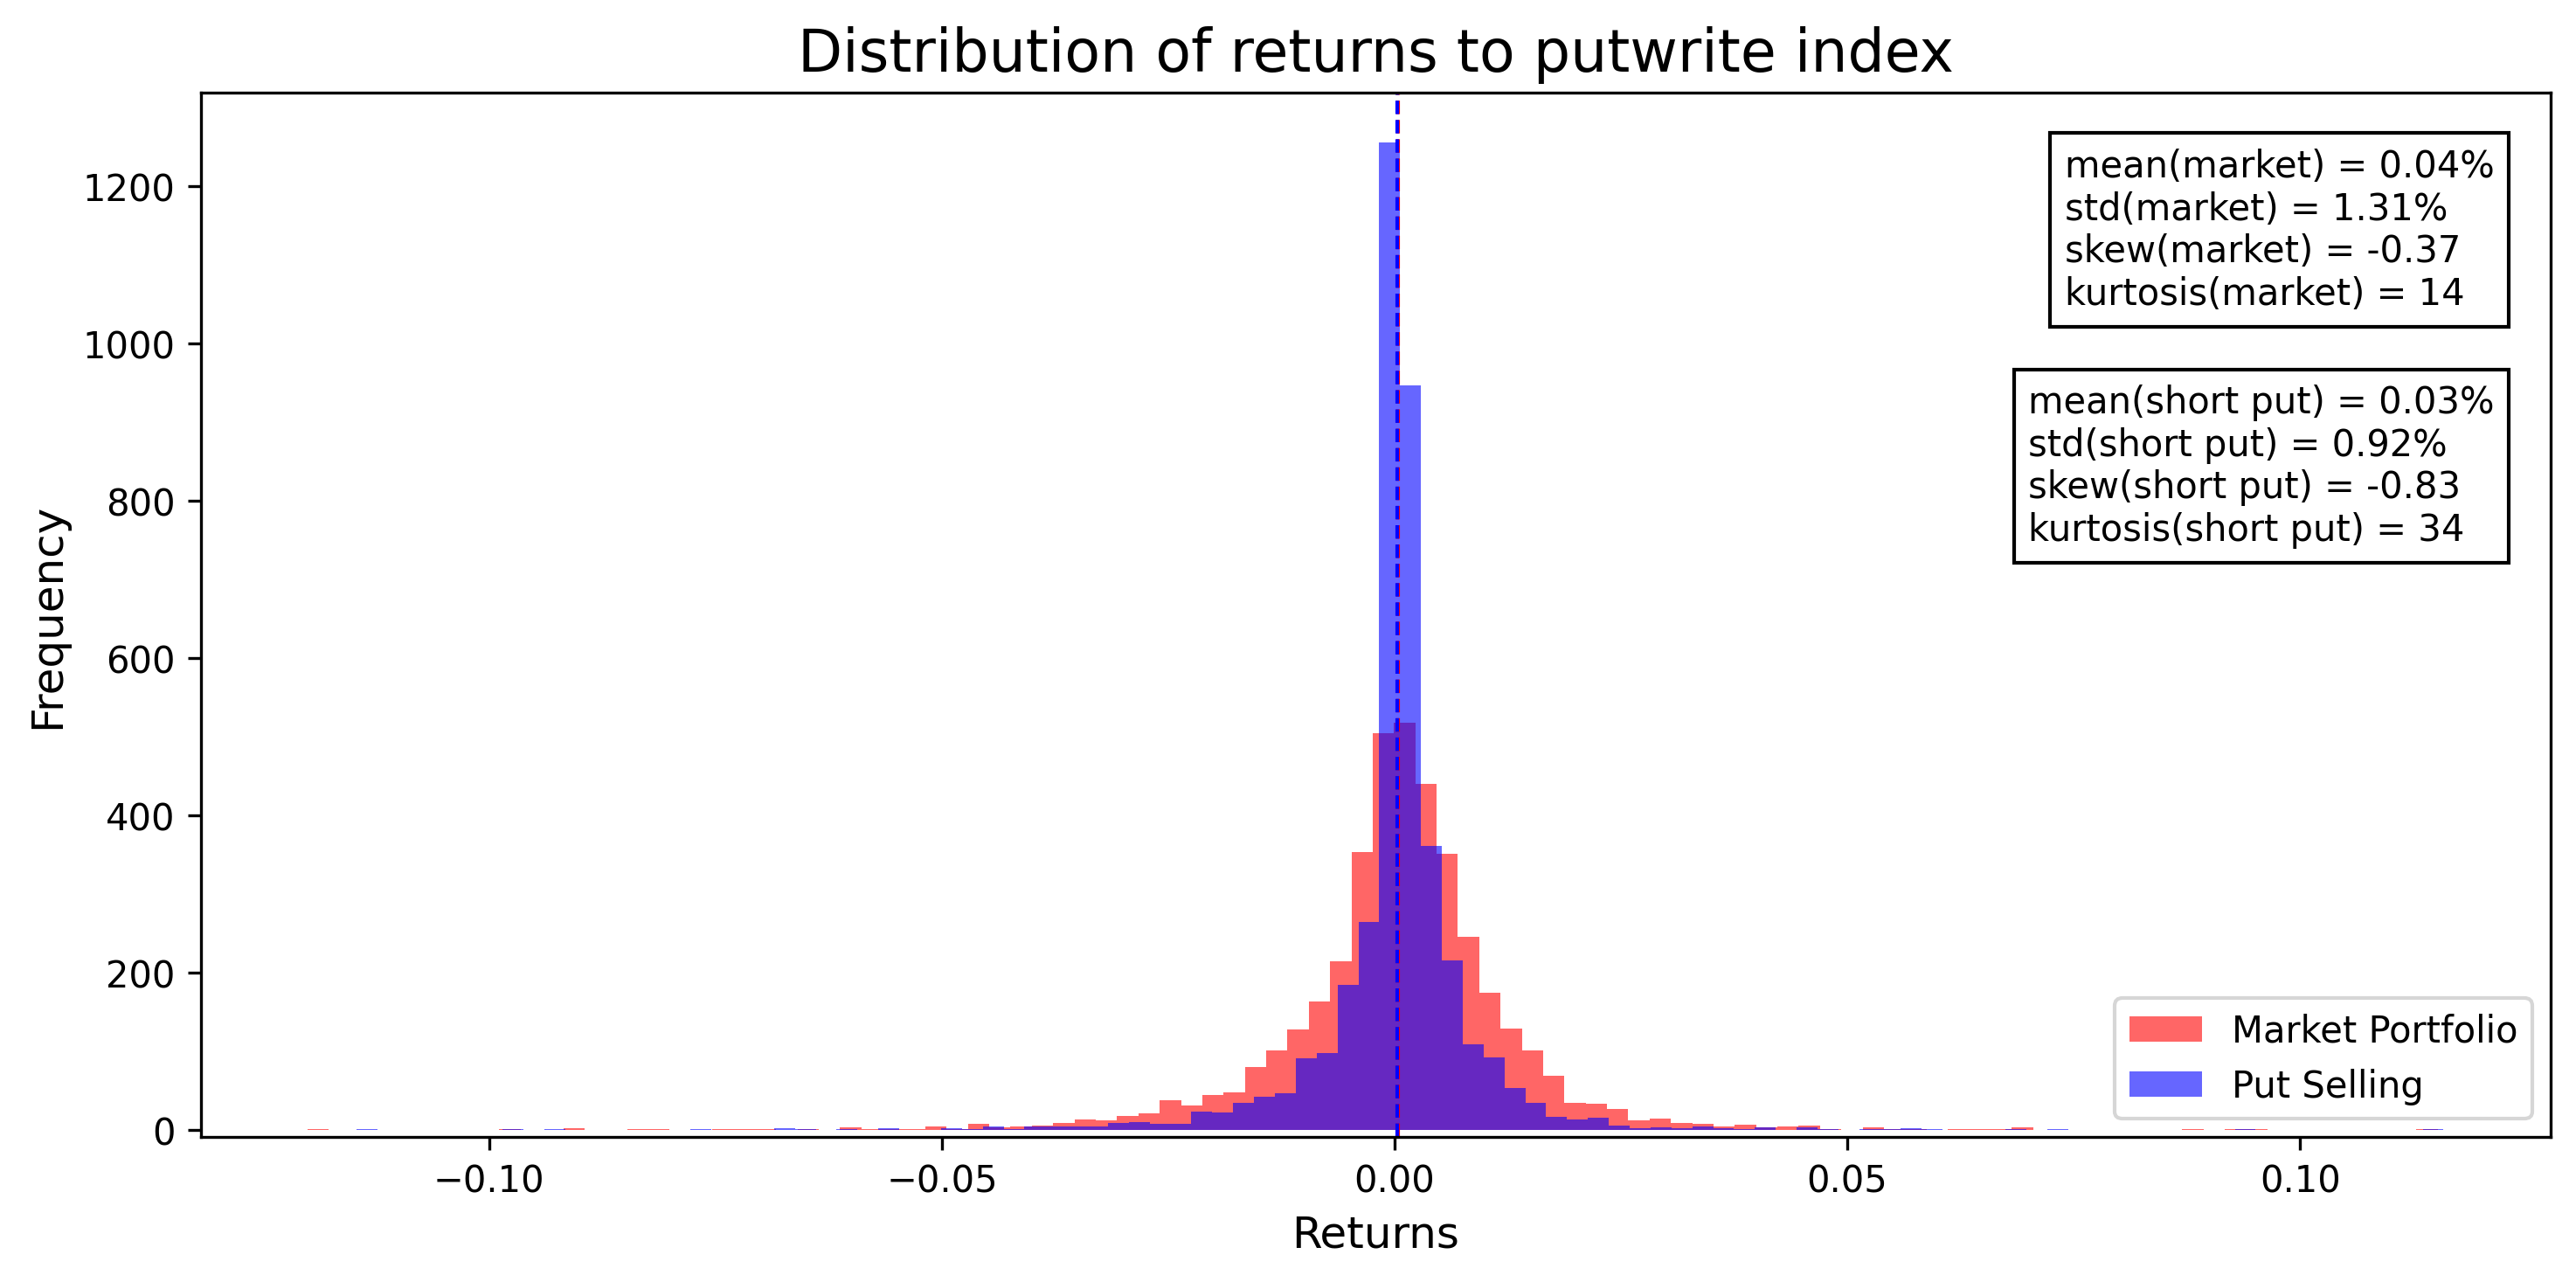
\includegraphics[width=0.75\textwidth]{fig13.png}
    \caption{Return distribution: S\&P 500 vs. PutWrite strategy}
    \label{fig:fig13}
\end{figure}

However, \autoref{fig:fig14} reveals the hidden danger. Examining the outliers (defined as daily returns with an absolute value above $3\%$), we find that the extreme losses are about the same in both cases. For very low stock returns, the put-write strategy behaves like leveraged stock exposure, yet unlike direct stock investment, investors are not conditioned to \say{expect the unexpected}.

\begin{figure}[h]
    \centering
    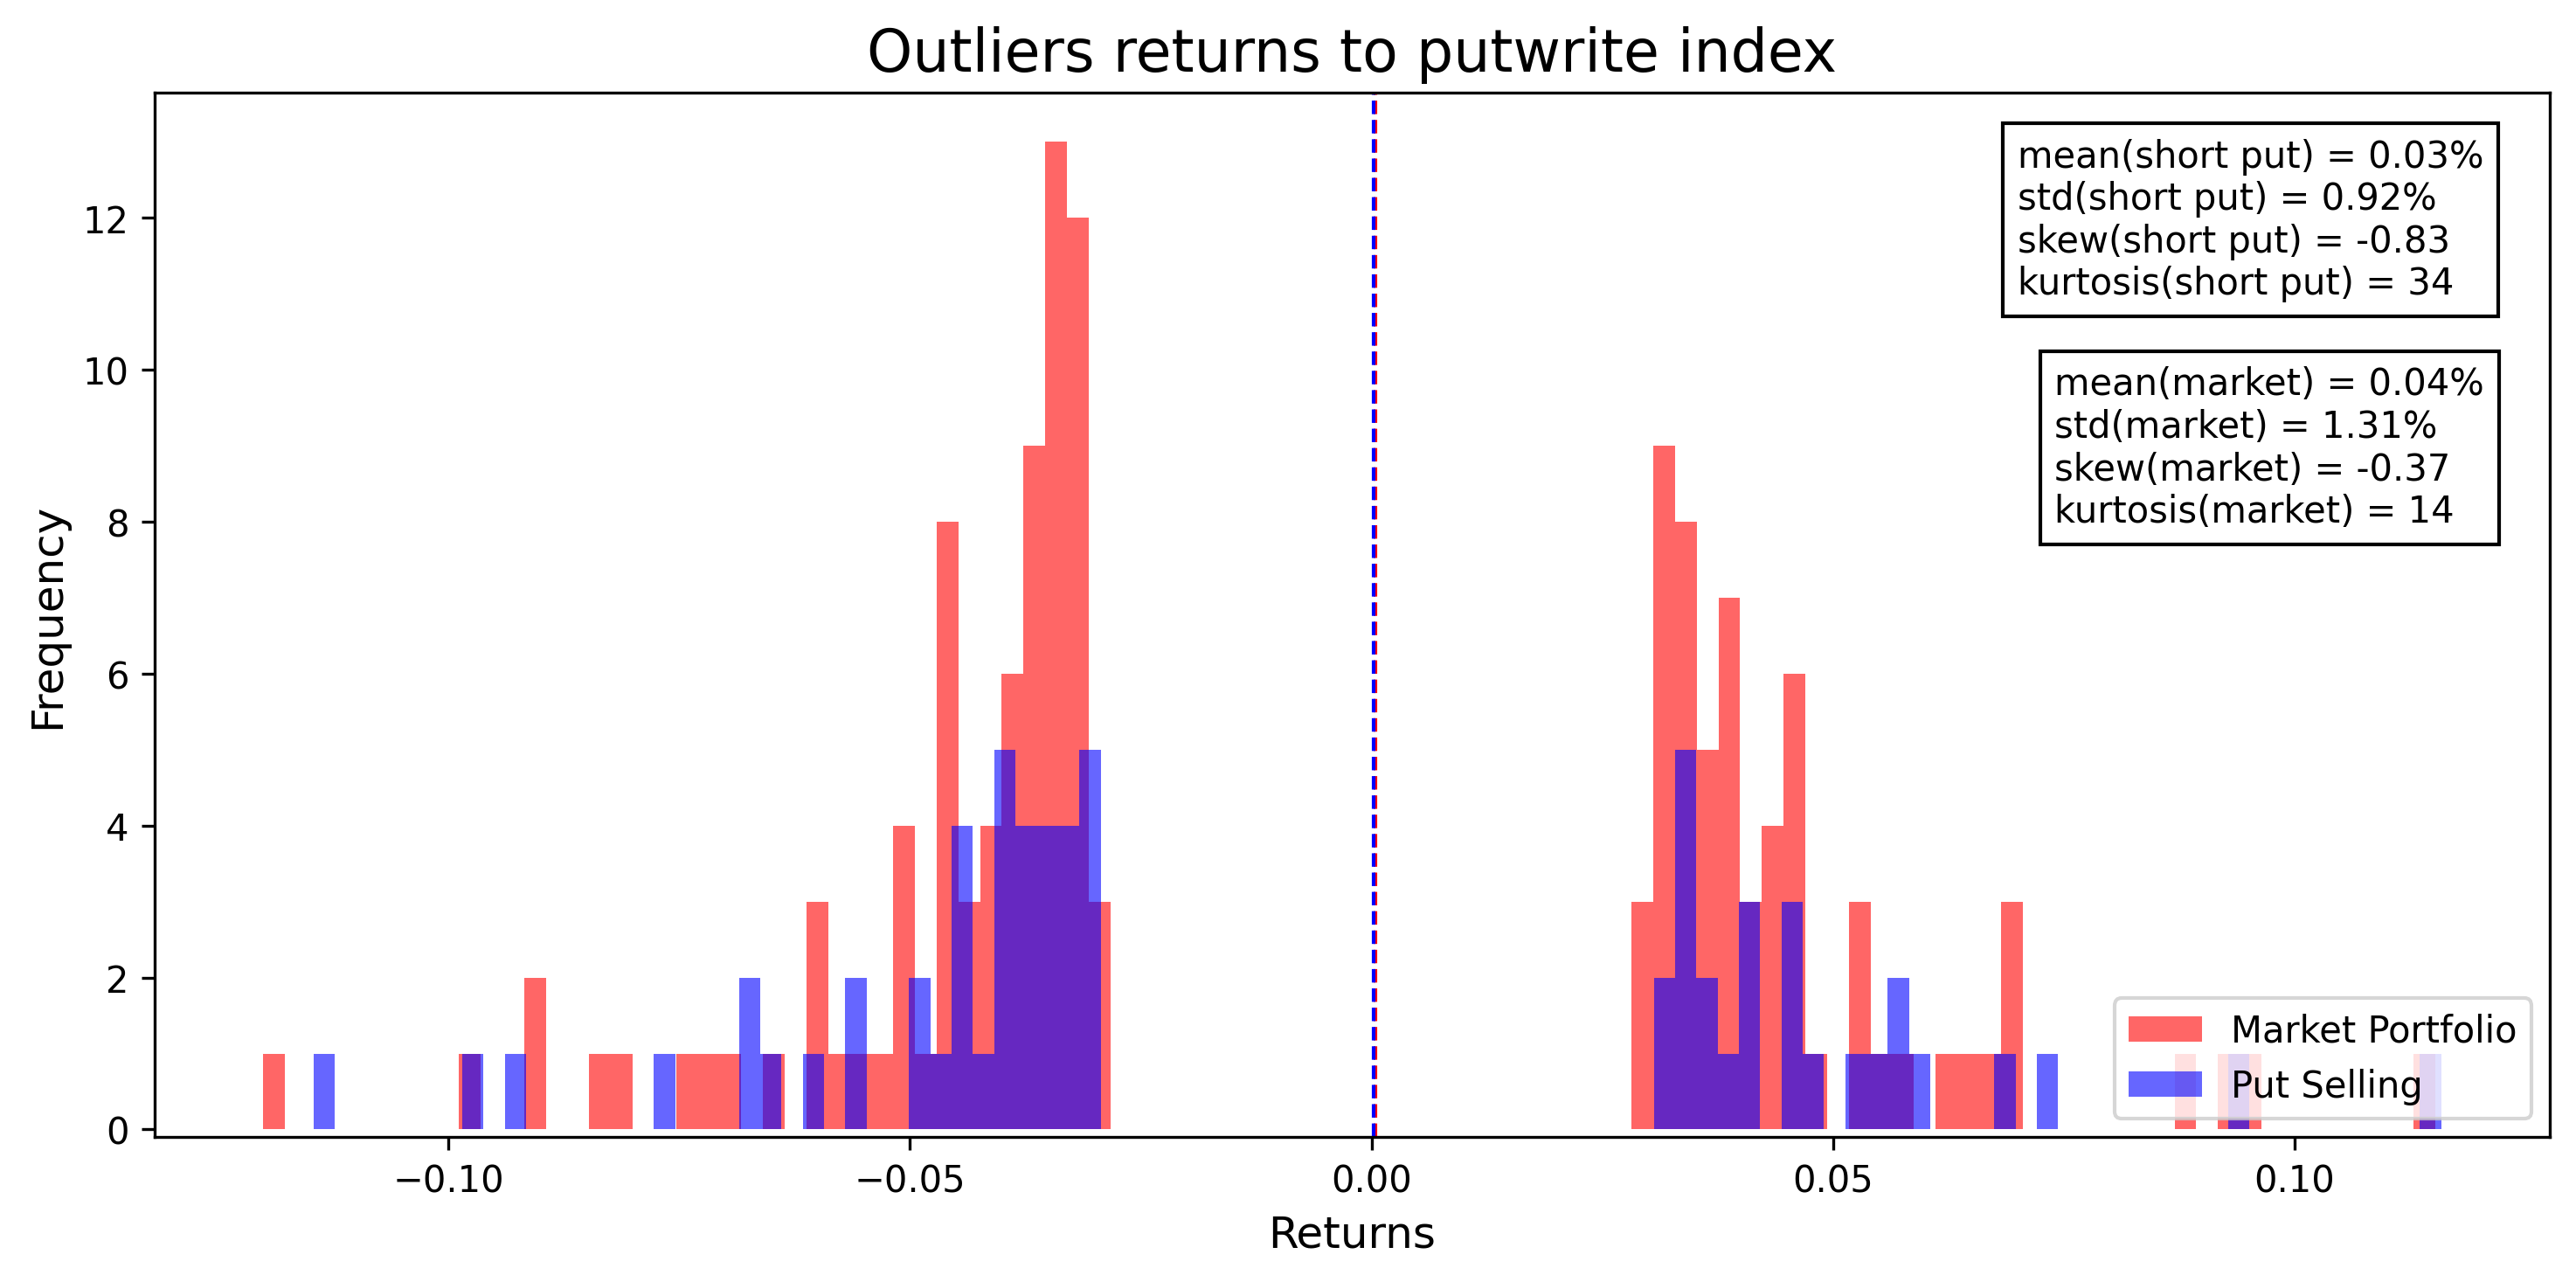
\includegraphics[width=0.75\textwidth]{fig14.png}
    \caption{Outlier returns}
    \label{fig:fig14}
\end{figure}

One might argue that sophisticated investors writing puts understand these risks and don't need such warnings. However, there is a deeper notion in which put options reveal the chicken narrative. First, the day-to-day payoffs represent the chicken before its neck is wrung, as steady small gains can mask hidden risk. The concentrated return distribution in Figure 13 shows this deceptive calm. Second, and more fundamentally, investors fell victim to the same type of model failure we saw in Section 5.2. Despite evidence of fat tails, many continued to rely on lognormal distribution assumptions that systematically underestimated tail risk.

The strategy's statistical properties (i.e., high frequency of small gains punctuated by rare large losses) are psychologically designed to encourage overconfidence in empirical patterns. Even sophisticated investors can fall prey to the same inductive reasoning that doomed Russell's chicken. They ignored the uncertainty outside their models and, as a result, were unprepared when that uncertainty manifested.


\subsection{The Chicken Problem is Everywhere}
The chicken problem extends beyond put options to other financial instruments with similar payoff structures.

Many accounts of the 2008-2009 crisis stress the role of credit default swaps. Market participants use credit default swaps to insure against default of a single entity, like a large financial institution, or baskets of corporate entities. Similar to life insurance, the protection buyer pays a periodic premium (called the spread) until maturity or default, and if the reference entity suffers a credit event, the writer compensates the buyer for the loss.

The CDX is an index of credit default swaps where market participants wrote contracts, known as tranches, that paid off depending on how many constituents of the CDX defaulted. The most super-senior of these tranches would only be affected if a large set of firms in the index defaulted simultaneously. 

\autoref{fig:fig15} \citep{seo2018rare} shows the time series of spreads on CDX super-senior tranches. Notice how spreads remained in the single digits from the onset of data availability through mid-2007, at which point they climbed as high as 80 basis points, increasing in 10-fold before 2008. This dramatic increase reflected a fundamental reassessment of systemic risk that market participants had previously underestimated. While some variation in spreads is expected, this pattern provides evidence that few market participants factored in the probability of an economy-wide crisis. Once again, steady returns on an asset that served as a substitute for cash lured investors into ignoring tail risk. Once again, an event outside of the model took market participants by surprise. 

\begin{figure}[h]
    \centering
    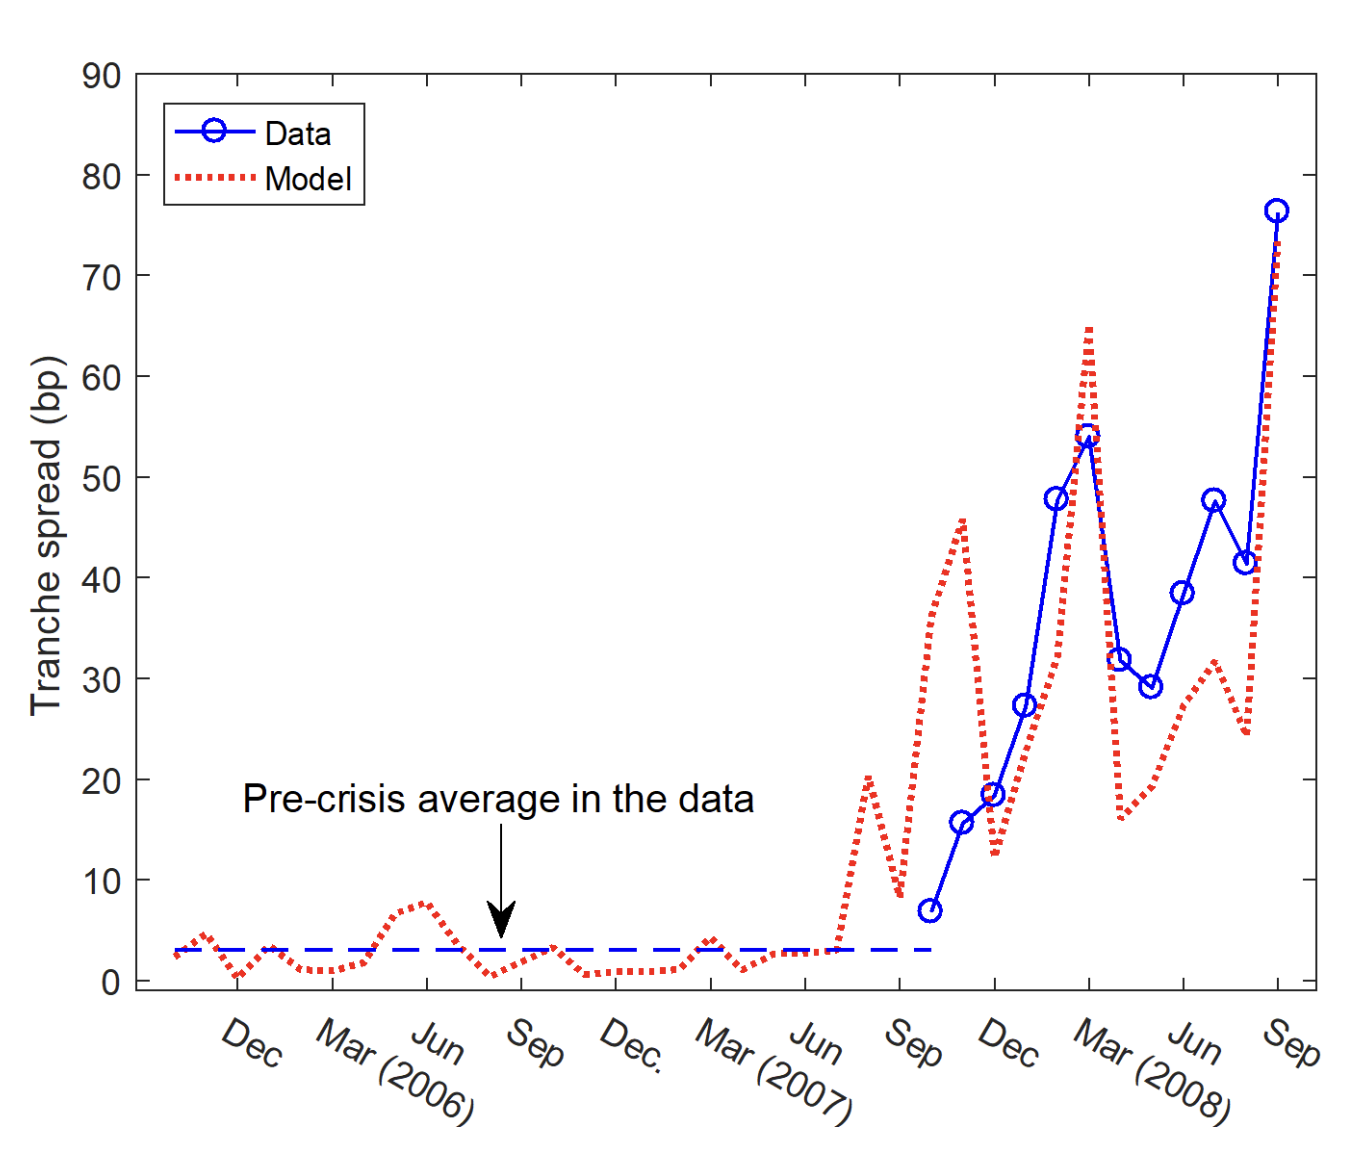
\includegraphics[width=0.75\textwidth]{fig15.png}
    \caption{Super-senior CDX spreads pre- and post-crisis \citep{seo2018rare}}
    \label{fig:fig15}
\end{figure}

Super-senior tranches exhibit the same deceptive pattern as Russell’s chicken: years of steady, small spreads followed by sudden catastrophic losses. Like put writers, investors collected modest premiums while remaining exposed to devastating tail events they systematically underpriced. 

The chicken problem extends even further through the fundamental structure of debt itself. Put-call parity shows that holding debt is mathematically equivalent to combining a risk-free bond with a short put position. Specifically, $\text{Debt} = \text{Riskless Bond} - \text{Put Option}$. Debt holders are essentially short put writers on the firm’s assets. If a firm’s value falls below the face value of its debt, debt holders suffer losses (exactly like put option writers when the underlying falls below the strike). Thus, put-like payoffs apply to all forms of lending: corporate bonds, bank deposits, short-term funding, and any other debt instrument. 

These embedded put options create interconnected vulnerabilities throughout the financial system. Short-term debt amplifies this problem through run dynamics. When concerns about solvency arise, creditors can withdraw funding quickly, forcing fire sales and creating the very losses that they feared.

This reveals why financial crises spread so quickly and broadly. The 1987 options market crash exposed a fundamental structure present throughout finance. Wherever there are promises to pay fixed amounts (debt), there are hidden put options. The chicken problem, with its deceptive pattern of steady gains masking tail risks, is not an anomaly but rather an inherent feature of modern financial systems.

The lesson from Russell's chicken applies far beyond any single strategy: when steady feeding suddenly stops, the consequences can be catastrophic and system-wide.